% !TeX root = RJwrapper.tex
\title{tmap: An R Package for thematic maps}
\author{by Martijn Tennekes}

\maketitle

\abstract{
A thematic map is a geographical map in which statistical data are visualized. The theme refers to the statistical phenomena that is shown, such as the unemployment rate at municipal level. 
The best known thematic map type is the choropleth, where regions are coloured according to a statistical variable, for instance unemployment rate or population density. Another popular thematic map type is the bubble map, in which the sizes of the bubbles are defined by a statistical variable, for instance city population.

With the tmap package, thematic maps can be generated with great flexibility. A thematic map is created by stacking layers, for instance one for colouring municipalities, one for thick borders of higher level regions, and one for text labels. 

The standard work flow that is needed to create a thematic map is embedded in tmap by several convenient functions for reading, appending, and transforming spatial data.
}

Introductory section which may include references in parentheses
\citep{R}, or cite a reference such as \citet{R} in the text.


\section{Introduction}



Bla bla bla test \citet{tmap} and \citep{sp2}. 


%This section may contain a figure such as Figure~\ref{figure:rlogo}.
%
\begin{widefigure}[htbp]
  \centering
  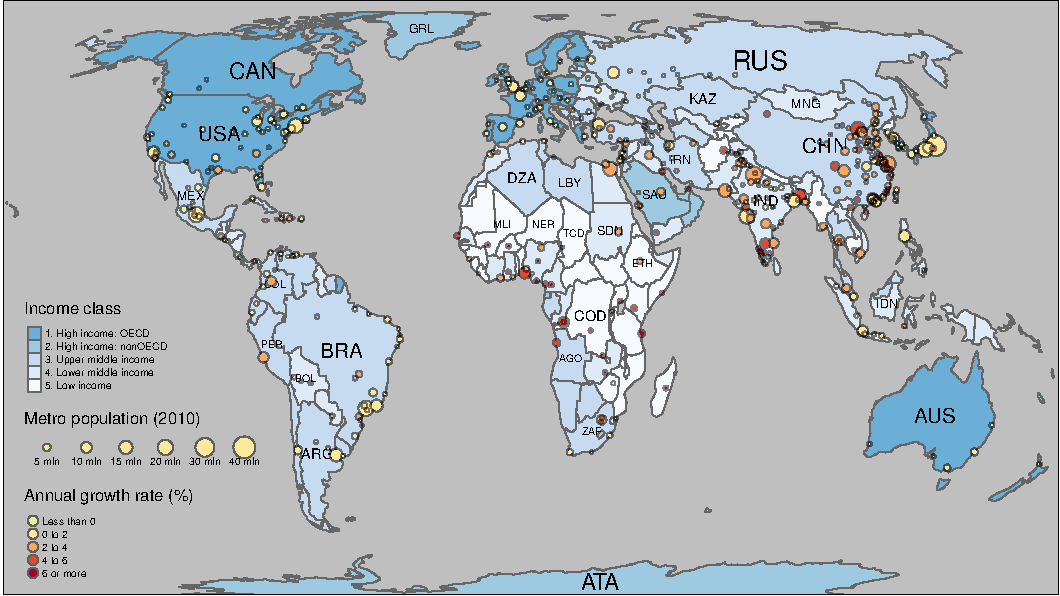
\includegraphics{bubbleMap2}
  \caption{Bubble map.}
  \label{figure:bubblemap}
\end{widefigure}

\section{Another section}

There will likely be several sections, perhaps including code snippets, such as:

\begin{example}
library(tmap)
data(Europe)
qtm(Europe)
\end{example}

\section{Summary}

This file is only a basic article template. For full details of \emph{The R Journal} style and information on how to prepare your article for submission, see the \href{http://journal.r-project.org/latex/RJauthorguide.pdf}{Instructions for Authors}.


\address{Martijn Tennekes\\
  Statistics Netherlands\\
  CBS-Weg 11, 6412 EX Heerlen\\
  Netherlands\\}
\email{mtennekes@gmail.com}

\bibliography{tennekes}
